\chapter{Implementation}
\label{chapter:implementation}

In this section there is a description of the implemented solution: hardware in the \autoref{sec:impl_hardware}, used software tools in the \autoref{sec:impl_software} and integration of all parts together in the \autoref{sec:impl_integration}. The code can be found on GitHub: stereo pair driver\footnote{\url{https://github.com/Myralllka/UAV_basler_stereopair_driver}} and the main module\footnote{\url{https://github.com/Myralllka/UAV_localisation_from_cameras}}.

\section{Hardware}
\label{sec:impl_hardware}
\begin{figure}[h]
  \begin{subfigure}[b]{0.49\textwidth}
    \centering
    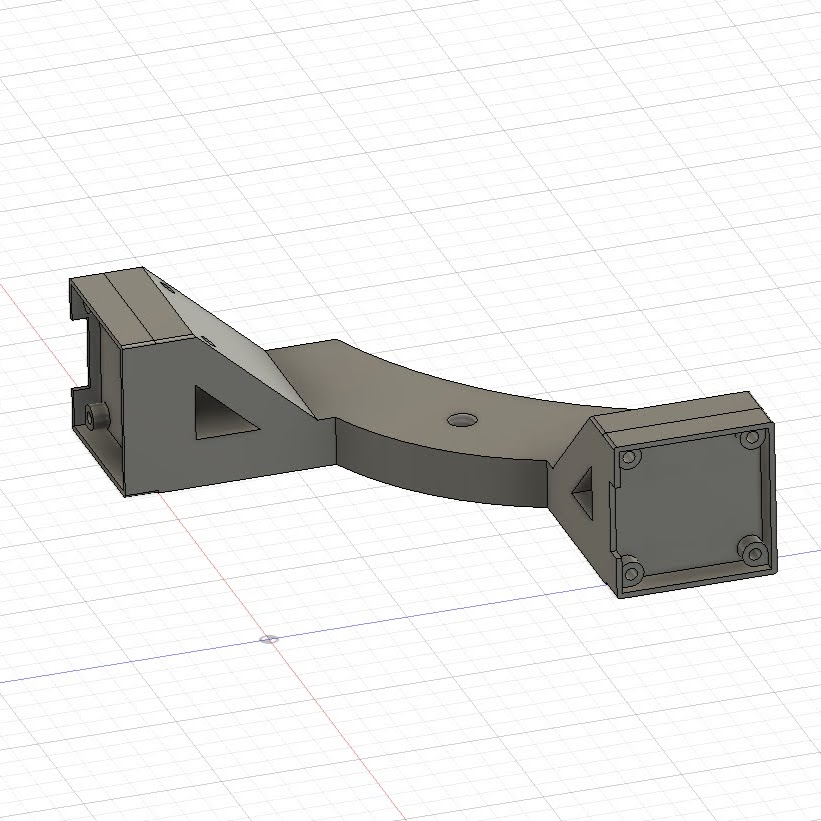
\includegraphics[width=\textwidth]{graphics/CAD.jpg}
    \caption{The CAD model of the prototype}
    \label{fig:proto_scheme}
  \end{subfigure}
  \hfill
  \begin{subfigure}[b]{0.49\textwidth}
    \centering
    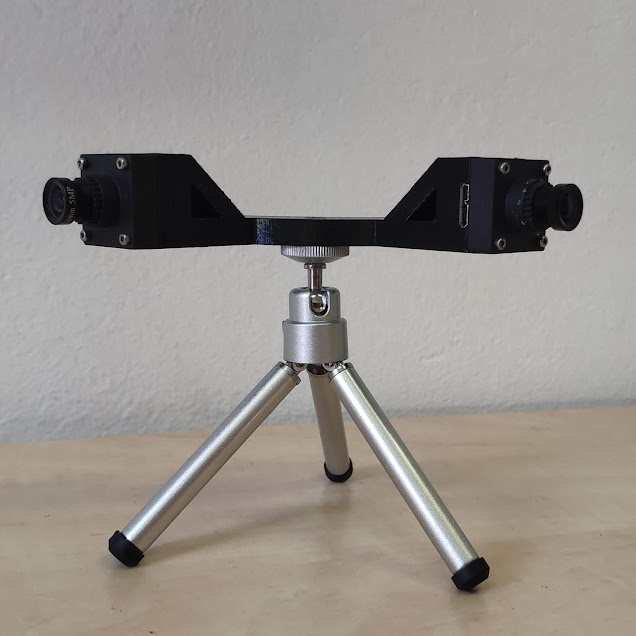
\includegraphics[width=\textwidth]{graphics/prototype.jpg}
    \caption{The printed prototype}
    \label{fig:proto_printed}
  \end{subfigure}
  \label{The proposed sollution prototype}
\end{figure}

The camera holder CAD model was created in a Fusion360 software considering requirements of rotation $90^\circ$ and the distance close to the average MAV sizes, the screenshot from modelling process is in \autoref{fig:proto_scheme}.
The 3d-printed solution prototype with cameras mounted is in the \autoref{fig:proto_printed}

Basler daA1600-60um cameras were chosen for this project because they have a global shutter to capture moving objects, good image quality and they are not so expensive.
\begin{center}
    \begin{tabular}{ l l }
    \hline
    name                   & property          \\ \hline
    Lens mount type        & S-mount           \\
    Data transfer protocol & USB 3.0           \\
    Max. frame rate        & 60 fps            \\
    Resolution (HxV)       & 1600 px x 1200 px \\
    Resolution             & 2 MP              \\
    Price                  & 289.00 EUR        \\ \hline
    \end{tabular}
\end{center}

Cameras' lences have $120^\circ$ FOV, which gives enough overlapping zone to detect features in $\sigma$ (see \autoref{fig:sch_stereo}).

Intel NUC with 8 cores CPU is used as the on-board computer for MAV. 
No external GPU is needed, so all algorithms should take it into consideration.

\section{Software tools}
\label{sec:impl_software}

The proposed solution uses Robotic operating system (ROS)\cite{Rospaper} as the middleware.
ROS is the whole ecosystem with hundrets of already implemented algorithms and libraries to interact with robots between Its parts and sensors.
It is an opensource tool, so the apriltag detector and camera driver used in this thesis are based on official modules from ROS community.

The MRS UAV system \cite{Baca2021} is used as a drone control environment. It is based on ROS, but it is the special framework for MAV's to implement and test path planning, control, computer vision, objects tracking and much more problems related to MAV's.
MRS lib\footnote{\url{https://ctu-mrs.github.io/mrs_lib/}} is a set of tools that make the process of using ROS more safe and simple.

OpenCV\footnote{\url{https://opencv.org/}} is an open-source library for computer vision.
Some of algorithms used in this thesis are taken from this library, PnP (\autoref{sec:pnp}) and improved version of triangulation from \autoref{sec:svdtriang} called "The Golden Standard Triangulation Method" which is a combination of SVD triangulation with applied Sampson correction.
Also feature detector and matcher (\autoref{sec:features}) both are used from the OpenCV.

Eigen\footnote{\url{https://eigen.tuxfamily.org/}} library is used for all linear algebra. 

\section{Integration}
\label{sec:impl_integration}

Implementation steps are described in the same order as in a \autoref{chapter:methodology}: calibrations, features matching, extracting 3D poses of features, error computation.

\begin{figure}[h]
    \centering
    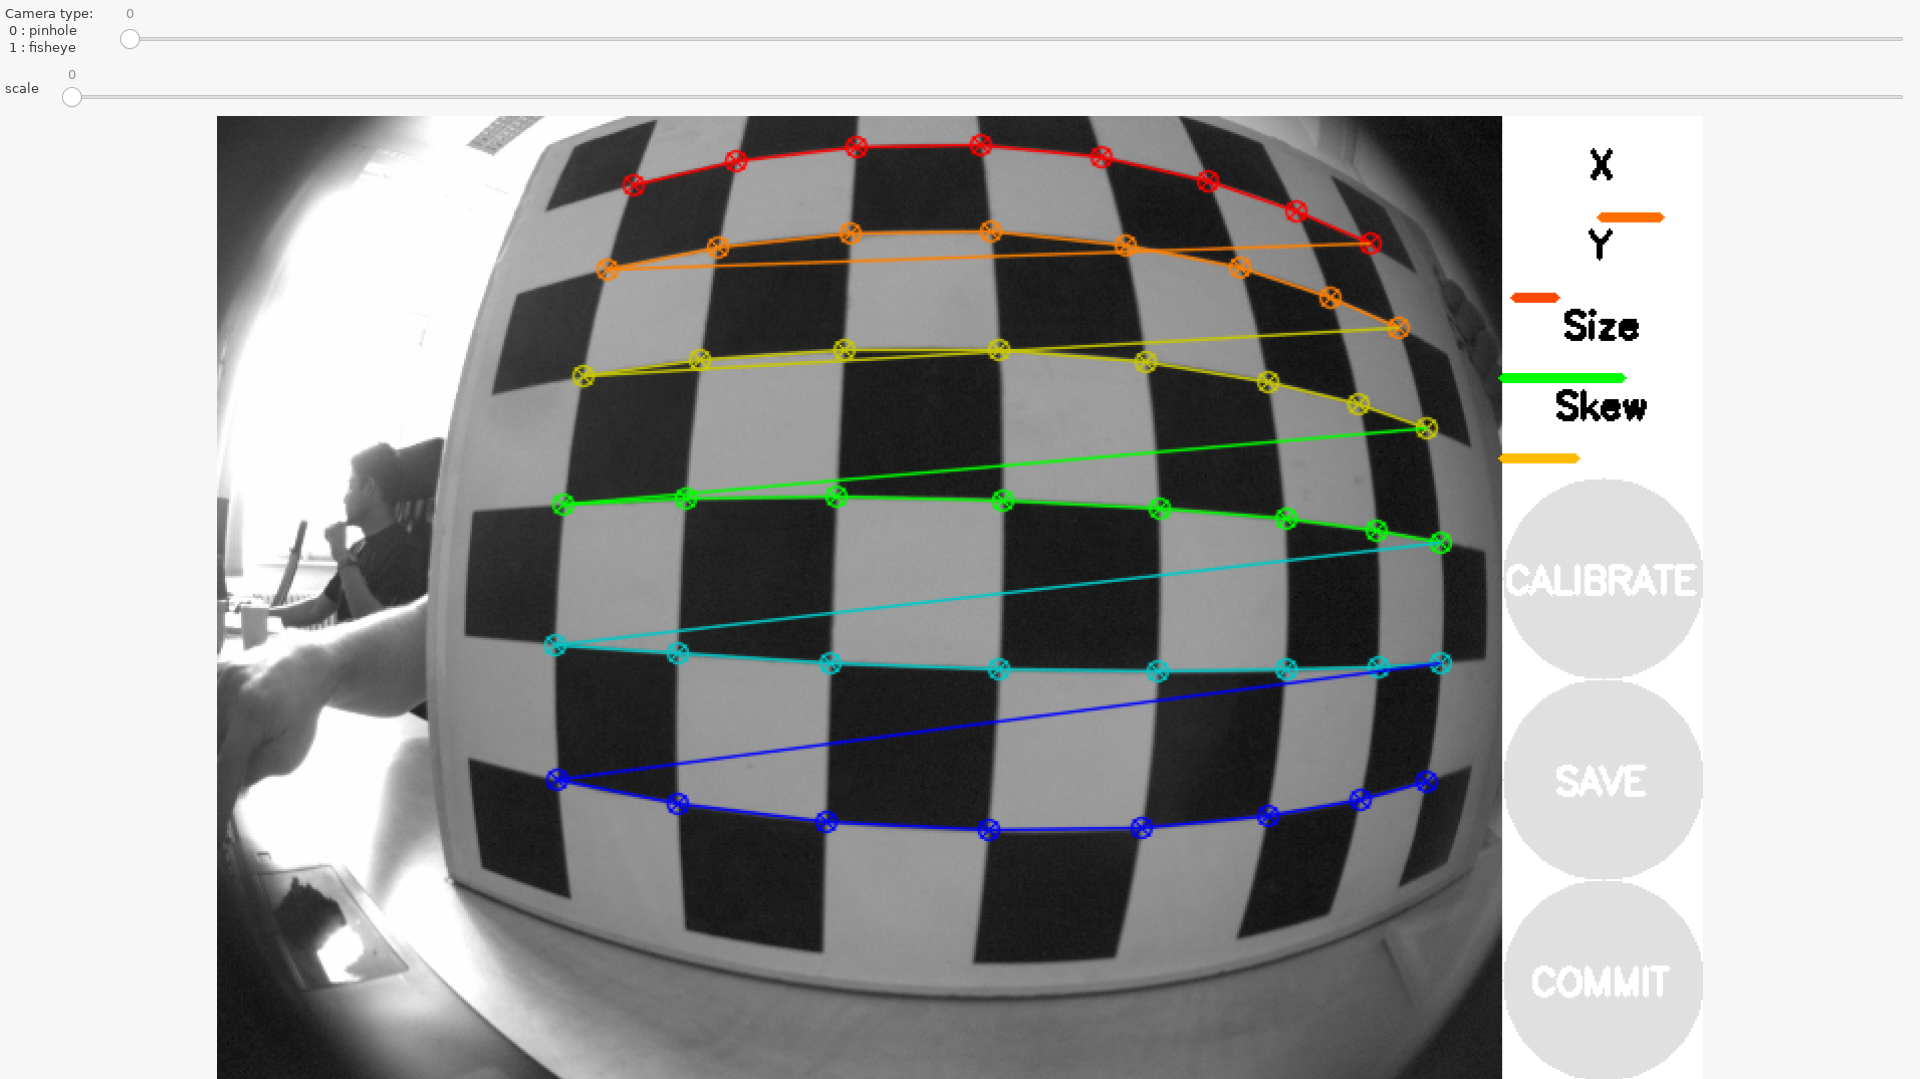
\includegraphics[width=.6\textwidth]{graphics/calibration.png}
    \caption{The calibration process}
    \label{fig:calib}
\end{figure}

There is a package\footnote{\url{http://wiki.ros.org/camera_calibration}} in ROS ecosystem, that can be used for the camera calibration (\autoref{sec:prelimin_calibration}). 
As input it takes a chessboard parameters (square size and number of squares) then in an interactive mode it collects images for calibration and as a result creates a file with camera calibration matrix and distortion coeficients, if the lens has a distortion.
The screenshot from the calibration application is in the \autoref{fig:calib}.

There are two implemented methods of a stereo pair calibration described in \autoref{sec:stereocalib}.
Both of them uses an apriltag calibration pattern.
The first method is implemented using the "Least-square estimation of transformation between two point sets" \cite{Umeyama1991} implementation from Eigen.
As the initial poses, measurements from the CAD model are used.
The second method is implemented using the OpenCV PnP solver.
As far as a standard apriltag detector outputs only the 3D poses of detected tags, it was modified to publish an external information needed for the PnP algorithm - 2D coordinates of apriltags' corners.




% Usage of proposed aproach: at a timestamp $t_1$ it is already possible to use SfM to make a point cloud from green + red points and blue + red.
% Here the proposed algorithm can help - it gives common points to an algorithm, so instead of SfM from 2 images it does SfM from 4 images but with bigger pressision, because $T_{static}$ remains the same, and the only necessary transformation that should be estimated is $T_{t_0t_1}$, and the innertial module can help with that.

% Another possible approach is to use already working SfM algorithm implementation for a left and rigth camera separately to obtaine two pointclouds, and then align them and fix a scale using Iterative closest point algorithm with respect to fixed red pointcloud
